\documentclass[11pt]{article}
\usepackage{arxiv}
\usepackage[utf8]{inputenc}
\usepackage[T1]{fontenc}
\usepackage{amsmath,amssymb,booktabs,array,microtype,graphicx,tabularx}
\usepackage[round]{natbib}
\usepackage[colorlinks=true,citecolor=blue,urlcolor=blue,linkcolor=blue]{hyperref}
\setlength{\emergencystretch}{2em}

\title{When Training-Only Risk Calibration Does Not Improve\\Element-Shift Prediction: A Frozen Negative Study}
\author{Ryan Gomez}
\date{October 21, 2026}

\newcommand{\method}{\textsc{Sparking}}
\newcommand{\dataset}{\texttt{matbench\_expt\_gap}}

\begin{document}
\maketitle

\begin{abstract}
Composition-only materials models can interpolate accurately while failing under
chemical support shift. We tested whether a training-only risk model could
identify when a five-seed CatBoost ensemble should be shrunk toward ridge
regression. The protocol was frozen before outcome-bearing execution. Within
each of three outer element exclusions (Cu, Ag, and B), eleven pseudo-element
exclusions generated harm labels without using outer-test targets. Four gate
temperatures were evaluated under a fixed selection rule. A private Kaggle run
completed 180 CatBoost GPU fits on dual Tesla T4 accelerators. Source and output
archives were hash-verified, all 18 hosted tests passed, and an independent
local verifier recomputed 156 metrics from retained predictions. The selected
gate ($T=0.40$ eV) achieved element-macro mean absolute error (MAE) of
0.779667 eV versus 0.779536 eV for the identical ungated ensemble, an
improvement of $-0.000130$ eV. The frozen admission criterion required an
improvement greater than 0.020 eV. The gate improved Ag and B by less than
0.001 eV each and worsened Cu by 0.001921 eV. Extra Trees was the strongest
control at 0.728675 eV macro MAE. A clearly labeled post hoc row-cluster
bootstrap gave a 95\% percentile interval of $[-0.001964,0.001428]$ eV for the
selected-gate effect. The scientific disposition is
\texttt{DEVELOPMENT\_\allowbreak{}NOT\_\allowbreak{}SUPPORTED}; protected Li, Zn, Ga, Se, and Te outcomes
were not opened. The result shows that moderate pseudo-shift harm ranking did
not translate into a practically useful adaptive gate under this frozen design.
\end{abstract}

\section{Introduction}
Composition-only property models are inexpensive screening surrogates, but they
omit crystal structure, defects, processing, and measurement context. Matbench
made several materials-learning tasks and splits reproducible
\citep{dunn2020matbench}; Magpie descriptors provide a widely used
composition-level representation \citep{ward2016magpie}. Learned composition
models such as Roost and CrabNet demonstrate substantial predictive utility
without structural input \citep{goodall2020roost,wang2021crabnet}. That utility
does not by itself establish reliability when a chemical element is absent from
training.

Domains-of-applicability studies document the degradation that can accompany
support shift \citep{sutton2020domains}, while redundancy-controlled evaluation
can expose optimistic interpolation estimates \citep{li2024mdhit}. A tempting
response is to estimate predictive risk from the training data and intervene
when risk is high. The difficult question is whether the estimated risk
transfers to the particular shift encountered at deployment.

We evaluate a narrow mechanism. A strong direct ensemble and a regularized
linear model are fit to the same target-independent descriptors. Pseudo-element
exclusions inside the outer training data teach a separate model to predict when
the direct ensemble has larger absolute error than ridge. Positive predicted
harm exponentially shrinks the direct prediction toward ridge. The study asks
whether this adaptive gate improves leave-one-element-out MAE relative to the
identical ungated ensemble.

The experiment was prospectively frozen after an earlier distance-gated version
showed negligible development benefit and diagnostic weaknesses. The successor
changed the representation, direct model, and gate, so it received a new
protocol and source identity. Its protected elements remained sealed behind a
conjunctive development rule. This report presents the complete verified
negative development result rather than continuing to search until a positive
gate appears.

\section{Methods}
\subsection{Dataset, representation, and outer shifts}
We use Matbench v0.1 \dataset{}, containing 4,604 formula--band-gap rows
\citep{dunn2020matbench}. The accepted compressed artifact has SHA-256
\texttt{783e7d14\allowbreak{}61eb83b0\allowbreak{}0b2f2942\allowbreak{}da4b95fd\allowbreak{}a5e58a0d\allowbreak{}1ae26b58\allowbreak{}1c24cf8a\allowbreak{}82ca75b2}.
The 270-dimensional target-independent representation concatenates 132 fixed
fraction and periodic-summary features with Magpie elemental-property statistics
and six stoichiometric norms. Missing values are imputed using the outer
training set only.

Development consists of three declared leave-one-element-out shifts. For element
$E$, every row containing $E$ forms the test set and is excluded from training.
The train/test counts are 4,214/390 for Cu, 4,408/196 for Ag, and 4,366/238 for
B. The three test sets have 824 memberships over 821 unique Matbench row
identifiers because a composition can contain more than one held-out element.
Li, Zn, Ga, Se, and Te are protected and were not evaluated.

\subsection{Direct model and controls}
The primary direct model is a five-seed CatBoost ensemble
\citep{prokhorenkova2018catboost}. Each member uses 1,200 iterations, depth 8,
learning rate 0.035, $\ell_2$ leaf regularization 5, random strength 0.5, border
count 128, and Bayesian bootstrap temperature 1.0. Predictions are clipped only
at zero and then averaged. The fixed seeds are 20261021 through 20261025.

Controls are the training median; standardized ridge with internally selected
regularization; direct squared-error histogram gradient boosting; a three-seed,
700-tree Extra Trees ensemble \citep{geurts2006extremely}; one CatBoost seed;
the five-seed CatBoost ensemble; and constant convex blends with direct weights
0.25, 0.50, and 0.75. Scikit-learn supplies ridge, histogram boosting, and Extra
Trees \citep{pedregosa2011scikit}. These controls separate adaptive gating from
ordinary shrinkage and from model-family choice.

\subsection{Training-only pseudo-exclusion calibration}
For each outer element, the gate is trained entirely within its outer training
set. Eleven declared pseudo elements---Na, Mg, Al, Si, P, Ca, Fe, K, Ti, Mn,
and Ni---are excluded one at a time. Ridge and the full five-seed CatBoost
ensemble predict each pseudo holdout. For row $i$, the harm target is
\begin{equation}
 h_i = |y_i-d_i|-|y_i-r_i|,
\end{equation}
where $d_i$ is the direct-ensemble prediction and $r_i$ is the ridge prediction.
Positive harm means ridge had smaller absolute error.

A histogram gradient-boosting regressor predicts harm from nine diagnostics.
They are the direct mean, ensemble standard deviation, ridge prediction,
direct--ridge disagreement, nearest-training distance, unseen-element fraction,
unseen-element count, composition element count, and fraction entropy. Each
pseudo element has equal total weight. The pseudo-calibration sets contain 2,069 rows for the Cu
outer model, 2,123 for Ag, and 2,105 for B.

Given predicted harm $\widehat h(x)$ and temperature $T$, the direct-model
weight and gated prediction are
\begin{align}
 w_T(x) &= \exp\!\left[-\frac{\max\{\widehat h(x),0\}}{T}\right],\\
 \widehat y_T(x) &= \max\{0,\ r(x)+w_T(x)[d(x)-r(x)]\}.
\end{align}
Thus nonpositive predicted harm preserves CatBoost, while positive predicted
harm shrinks continuously toward ridge. The complete temperature grid is
$T\in\{0.05,0.10,0.20,0.40\}$ eV.

\subsection{Frozen selection and stopping rule}
The primary metric is the unweighted mean of Cu, Ag, and B MAE. The numerical
minimum is identified first; candidates within 0.005 eV choose the largest
$T$, the least aggressive shrinkage. Protected confirmation is admitted only if
all of the following hold:
\begin{enumerate}
  \item selected-gate macro MAE improves over the identical ungated CatBoost
        ensemble by more than 0.020 eV;
  \item at least two of three development elements improve;
  \item the gate is active on 1--90\% of every element holdout;
  \item CatBoost predictions are nonconstant, every pseudo exclusion completes,
        and all retained evidence is finite and manifest-valid.
\end{enumerate}
The rule is conjunctive. Failure terminates v2 without opening protected
outcomes. The primary effect is
\begin{equation}
 \Delta = \frac{1}{3}\sum_E
 \left[\operatorname{MAE}_{E}(d)-\operatorname{MAE}_{E}(\widehat y_T)\right],
 \quad E\in\{\mathrm{Cu},\mathrm{Ag},\mathrm{B}\}.
\end{equation}
Positive values favor the gate.

\subsection{Evidence and computation}
The frozen source commit is
\texttt{5a56bb5d\allowbreak{}c9761973\allowbreak{}0f0fbc65\allowbreak{}44490cdc\allowbreak{}69f2c109}; the protocol SHA-256 is
\texttt{c4aa306c\allowbreak{}72592380\allowbreak{}75db18ce\allowbreak{}d236e99d\allowbreak{}59101d57\allowbreak{}321e733e\allowbreak{}84c458f2\allowbreak{}b7237c2e}.
The private Kaggle kernel ran Python 3.13.15, CatBoost 1.2.10, matminer 0.10.1,
and NumPy 2.5.4 on two Tesla T4 GPUs with 15,360 MiB each. The design requires
60 CatBoost fits per outer element: 11 pseudo exclusions times five seeds plus
five outer fits, for 180 fits total.

The run retained member predictions, pseudo-calibration rows, gate weights,
per-example predictions, aggregate metrics, feature schema, environment,
resource observations, GPU identities, and a content manifest. The published
archive checksum was verified before safe extraction. A separate local verifier
then checked all files and recomputed every reported metric from the arrays.

\subsection{Post hoc descriptive uncertainty}
The frozen gate decision uses the practical-effect rule above. After that
decision, we computed a descriptive 20,000-resample percentile bootstrap with
seed 20261021. The sampling unit is the unique Matbench row identifier across
all three holdouts; resampling a row therefore keeps its memberships coupled.
This analysis was not prospectively specified, and the three development
elements are selected scenarios rather than a random population of elements.
It is reported as a sensitivity description, not as a new decision rule.

\section{Results}
\subsection{Primary development decision}
All 180 GPU fits completed in 6,845.90 seconds. Peak host resident memory was
914.55 MiB and the pageout delta was zero. All 18 hosted tests passed. The gate
was active on 18.7\% of Cu, 13.3\% of Ag, and 19.3\% of B, satisfying the
nondegeneracy rule. CatBoost predictions were nonconstant, and all 33 declared
pseudo exclusions completed.

The selected $T=0.40$ gate achieved macro MAE 0.779667 eV; the ungated CatBoost
ensemble achieved 0.779536 eV. Hence $\Delta=-0.000130$ eV. Per-element effects
were $-0.001921$ eV for Cu, $+0.000967$ eV for Ag, and $+0.000563$ eV for B.
The sign-count condition passed, but the required $>0.020$ eV practical effect
failed. The prospectively frozen disposition is therefore
\texttt{DEVELOPMENT\_\allowbreak{}NOT\_\allowbreak{}SUPPORTED}.

The numerical minimum was $T=0.05$ at 0.776451 eV, a 0.003086 eV improvement
over CatBoost. It was within 0.005 eV of the $T=0.40$ candidate, so the tie rule
selected $T=0.40$. Neither candidate approached the admission threshold.

\begin{table}[t]
\centering
\caption{Development MAE (eV). Macro is the unweighted mean across elements.
The Extra Trees result is a secondary control; the frozen hypothesis concerns
the selected risk gate versus the identical CatBoost ensemble.}
\label{tab:development}
\resizebox{\linewidth}{!}{\begin{tabular}{lrrrr}
\toprule
Model & Cu & Ag & B & Macro \\
\midrule
Extra Trees ensemble & 0.7271 & 0.3708 & 1.0881 & 0.7287 \\
CatBoost single seed & 0.6978 & 0.4019 & 1.2164 & 0.7720 \\
Direct HGB & 0.6460 & 0.4395 & 1.2329 & 0.7728 \\
Risk gate, $T=0.05$ & 0.7078 & 0.3950 & 1.2266 & 0.7765 \\
CatBoost ensemble & 0.7095 & 0.3991 & 1.2300 & 0.7795 \\
Selected risk gate, $T=0.40$ & 0.7115 & 0.3981 & 1.2294 & 0.7797 \\
Ridge & 0.8021 & 0.5484 & 1.3216 & 0.8907 \\
\bottomrule
\end{tabular}
}
\end{table}

\begin{figure}[t]
\centering
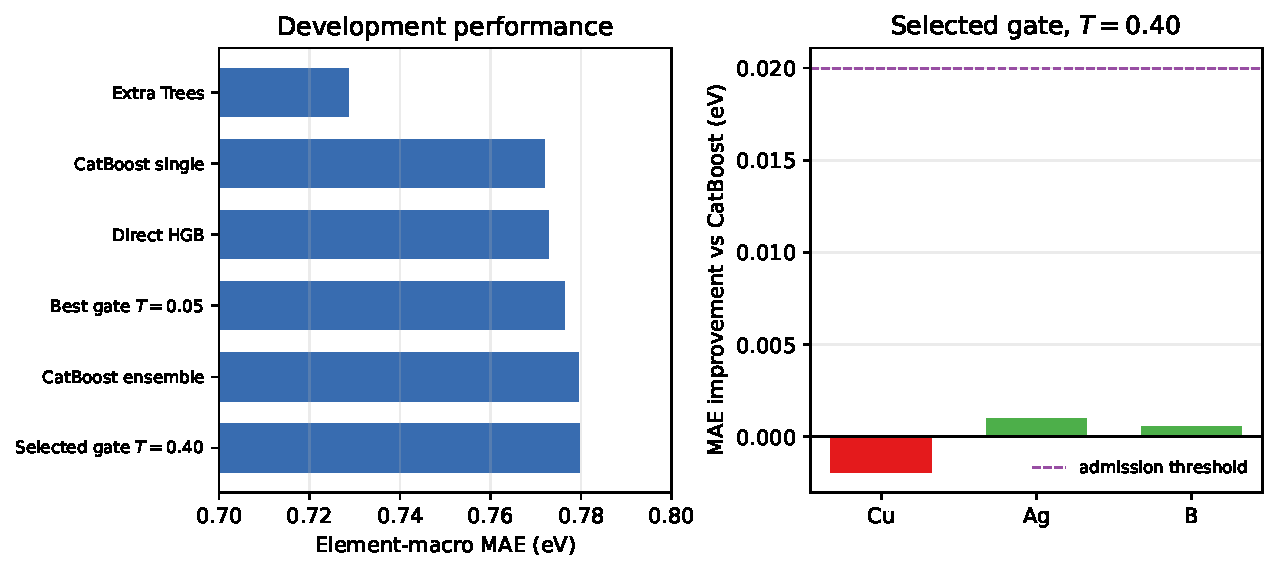
\includegraphics[width=\linewidth]{figures/development-v2-results.pdf}
\caption{Left: development macro MAE for principal models (axis begins at
0.70 eV). Right: selected-gate paired MAE improvements by element; positive
values favor the gate. The dashed line is the 0.020 eV macro admission
threshold, shown as a scale reference.}
\label{fig:development}
\end{figure}

\subsection{Controls and risk transfer}
Extra Trees was the best evaluated control at 0.728675 eV macro MAE, improving
by 0.050862 eV relative to the CatBoost ensemble. One CatBoost seed
(0.772015 eV) and direct histogram boosting (0.772843 eV) also outperformed the
five-seed CatBoost mean. These are development comparisons under the same three
shifts; they do not establish a leaderboard claim or authorize protected
evaluation.

The harm model's Spearman correlation on pseudo-calibration rows was 0.666 for
Cu, 0.656 for Ag, and 0.707 for B. On the actual outer holdouts, descriptive
risk--harm correlations fell to 0.309, 0.527, and 0.240. The gate therefore
learned nontrivial ordering within pseudo shifts, but that ordering transferred
weakly and inconsistently to the declared outer shifts.

\begin{table}[h]
\centering
\caption{Risk-calibration diagnostics. Outer correlations are descriptive
because outer targets participate in evaluation.}
\label{tab:risk}
\begin{tabular}{lrrr}
\toprule
Outer element & Pseudo rows & Pseudo Spearman & Outer Spearman \\
\midrule
Cu & 2,069 & 0.666 & 0.309 \\
Ag & 2,123 & 0.656 & 0.527 \\
B  & 2,105 & 0.707 & 0.240 \\
\bottomrule
\end{tabular}
\end{table}

\subsection{Post hoc uncertainty description}
The row-cluster bootstrap interval for the selected-gate macro improvement was
$[-0.001964,0.001428]$ eV. The fraction of bootstrap replicates above zero was
0.4596; none of 20,000 exceeded 0.020 eV. Paired-row intervals were
$[-0.006702,0.001790]$ eV for Cu, $[-0.001664,0.003509]$ eV for Ag, and
$[-0.000391,0.001447]$ eV for B. These descriptive intervals agree with the
primary conclusion that any effect under this development design is tiny
relative to the declared practical threshold.

\subsection{Independent verification}
Kaggle reported the kernel terminal state as complete. The source roundtrip
matched 40 files with no missing, extra, or changed entries. The output archive
SHA-256 was
\texttt{cf8aeceb\allowbreak{}f1dec60c\allowbreak{}cfb48445\allowbreak{}b25a891b\allowbreak{}75b2feff\allowbreak{}7fb37cf0\allowbreak{}e08774fb\allowbreak{}deeb420a}.
Its 18 members had no absolute paths, traversal components, links, or device
entries. All 17 extracted run files matched the direct Kaggle download
byte-for-byte; their retained tree digest was
\texttt{43eb835f\allowbreak{}5fe7eef6\allowbreak{}82502fee\allowbreak{}15c3e6fd\allowbreak{}33265873\allowbreak{}13fd2a93\allowbreak{}a6a5fe39\allowbreak{}8cf32c5c}.
The independent verifier found a valid manifest and reproduced 156 metric
comparisons. Both hosted and local verification confirmed that protected and
official-fold outcomes were absent.

\section{Discussion}
The result separates risk ranking from useful intervention. Pseudo-exclusion
correlations of roughly 0.66--0.71 show that the harm model captured structure
in its constructed calibration set. The much smaller outer correlations and
near-zero MAE effects show that this structure did not support a practically
valuable gate on Cu, Ag, and B. A risk score can be statistically ordered yet
still fail to improve the downstream decision.

The constant-blend controls also matter. They performed worse than CatBoost,
which means indiscriminate shrinkage toward ridge was harmful. The adaptive gate
avoided most of that damage, but avoidance is not improvement. Meanwhile Extra
Trees substantially outperformed the CatBoost ensemble on these development
shifts, suggesting that model-family robustness was more consequential than the
proposed risk correction in this experiment.

The pseudo-exclusion data include extreme ridge failures, especially for Fe.
Because pseudo elements received equal total weight, those retained cases may
have shaped the learned harm surface. Removing, clipping, or reweighting them
after observing the result would be a new hypothesis. Such work must use a new
versioned protocol and cannot reinterpret v2 as successful.

\section{Limitations and Claim Boundary}
Only three development elements were evaluated, and their test sets overlap.
They are fixed stress scenarios, not a random sample of chemical elements, so
neither the bootstrap nor the sign count supports population-wide inference.
Composition-only descriptors cannot resolve polymorphs, defects, processing,
or measurement context. The public dataset itself may contain redundancy, and
leave-one-element-out shift does not represent every deployment shift.

GPU boosting can vary with floating-point reduction order. We retained all five
member predictions and report the executed ensemble rather than claiming
byte-identical retraining. Hyperparameters were fixed and no protected outcome
was used, but selecting among four temperatures on three outer scenarios can
still overfit development. The admission threshold was intended to prevent a
small selected fluctuation from reaching confirmation.

The result supports one bounded conclusion: the frozen v2 risk gate did not
justify protected confirmation on Cu/Ag/B. It does not prove that risk gating is
universally ineffective, that Extra Trees is state of the art, or that any model
identifies stable, synthesizable, safe, novel, or useful materials. No v2 claim
is available about official Matbench-fold preservation or the protected Li, Zn,
Ga, Se, and Te shifts.

\section{Conclusion}
A fully executed, hash-verified GPU experiment found no practically meaningful
benefit from training-only risk-gated shrinkage of a CatBoost ensemble. The
selected gate slightly worsened macro MAE, and even the numerically best gate
fell far below the prospectively frozen improvement threshold. The correct
scientific action is to retain the negative result and stop before protected
confirmation. This outcome narrows future work toward better shift proxies,
robust treatment of pathological pseudo exclusions, and model-family choices,
all under separately versioned protocols.

\section*{Reproducibility and Artifact Statement}
The retained package contains the frozen protocol; exact source commit and
archive digests; raw outer predictions; five CatBoost members per element;
pseudo-calibration arrays; per-example risk features and gate weights; GPU
admission and postflight receipts; environment freeze; resource trace; kernel
log; aggregate results; and a manifest. The private Kaggle output was downloaded
from kernel version 1 and independently verified locally. The deterministic
secondary analysis regenerates Table~\ref{tab:development},
Figure~\ref{fig:development}, and the post hoc uncertainty receipt. At the time
of this report, the hosted kernel and dataset are private; the retained local
artifacts are the review record and are not described as independently public.

\section*{Data and Ethics Statement}
The study uses the previously published Matbench experimental-gap benchmark and
contains no human participants or personal data. It makes no recommendation to
synthesize or deploy a material. Experimental validation, safety assessment,
and application-specific review remain necessary for any downstream use.

\bibliographystyle{plainnat}
\bibliography{references}

\appendix
\section{Frozen Identity and Decision Matrix}
\begin{tabularx}{\linewidth}{>{\raggedright\arraybackslash}p{0.32\linewidth}X}
\toprule
Item & Value \\
\midrule
Study & \texttt{sparking-development-v2-}\allowbreak{}\texttt{risk-gated-gpu} \\
Run & \texttt{kaggle-development-v2-r1} \\
Source commit & {\footnotesize\texttt{5a56bb5d\allowbreak{}c9761973\allowbreak{}0f0fbc65\allowbreak{}44490cdc\allowbreak{}69f2c109}} \\
Protocol digest & {\footnotesize\texttt{c4aa306c\allowbreak{}72592380\allowbreak{}75db18ce\allowbreak{}d236e99d\allowbreak{}59101d57\allowbreak{}321e733e\allowbreak{}84c458f2\allowbreak{}b7237c2e}} \\
Selected model & risk gate, $T=0.40$ eV \\
Primary effect & $-0.000130$ eV \\
Required effect & $>0.020$ eV \\
Disposition & \texttt{DEVELOPMENT\_\allowbreak{}NOT\_\allowbreak{}SUPPORTED} \\
Protected outcomes & unopened \\
\bottomrule
\end{tabularx}

\section{Exact Verification Commands}
\begin{verbatim}
.venv/bin/python scripts/verify_successor_v2.py \
  runs/kaggle-development-v2-r1
MPLCONFIGDIR=/tmp/sparking-matplotlib \
  .venv/bin/python scripts/analyze_successor_v2.py
\end{verbatim}

\end{document}
